\documentclass[border=4pt]{standalone}
\usepackage[T1]{fontenc}
\usepackage{helvet}
\renewcommand{\familydefault}{\sfdefault}
\usepackage{tikz}
\usetikzlibrary{positioning,arrows.meta,calc,fit,backgrounds}
\definecolor{ink}{HTML}{2C3138}
\definecolor{ink2}{HTML}{52514E}
\definecolor{pblue}{HTML}{EAF3FC}
\definecolor{pblueline}{HTML}{7CB6F1}
\definecolor{prose}{HTML}{FBEDEB}
\definecolor{proseline}{HTML}{D99A93}
\definecolor{pgreen}{HTML}{EEF6E9}
\definecolor{pgreenline}{HTML}{94C07C}
\definecolor{plav}{HTML}{F1ECFB}
\definecolor{plavline}{HTML}{B59BE6}
\definecolor{papri}{HTML}{FCF1E9}
\definecolor{papriline}{HTML}{E3A072}
\definecolor{pgold}{HTML}{F8F3E4}
\definecolor{pgoldline}{HTML}{CBAE5E}
\definecolor{pband}{HTML}{F3F4F6}
\begin{document}
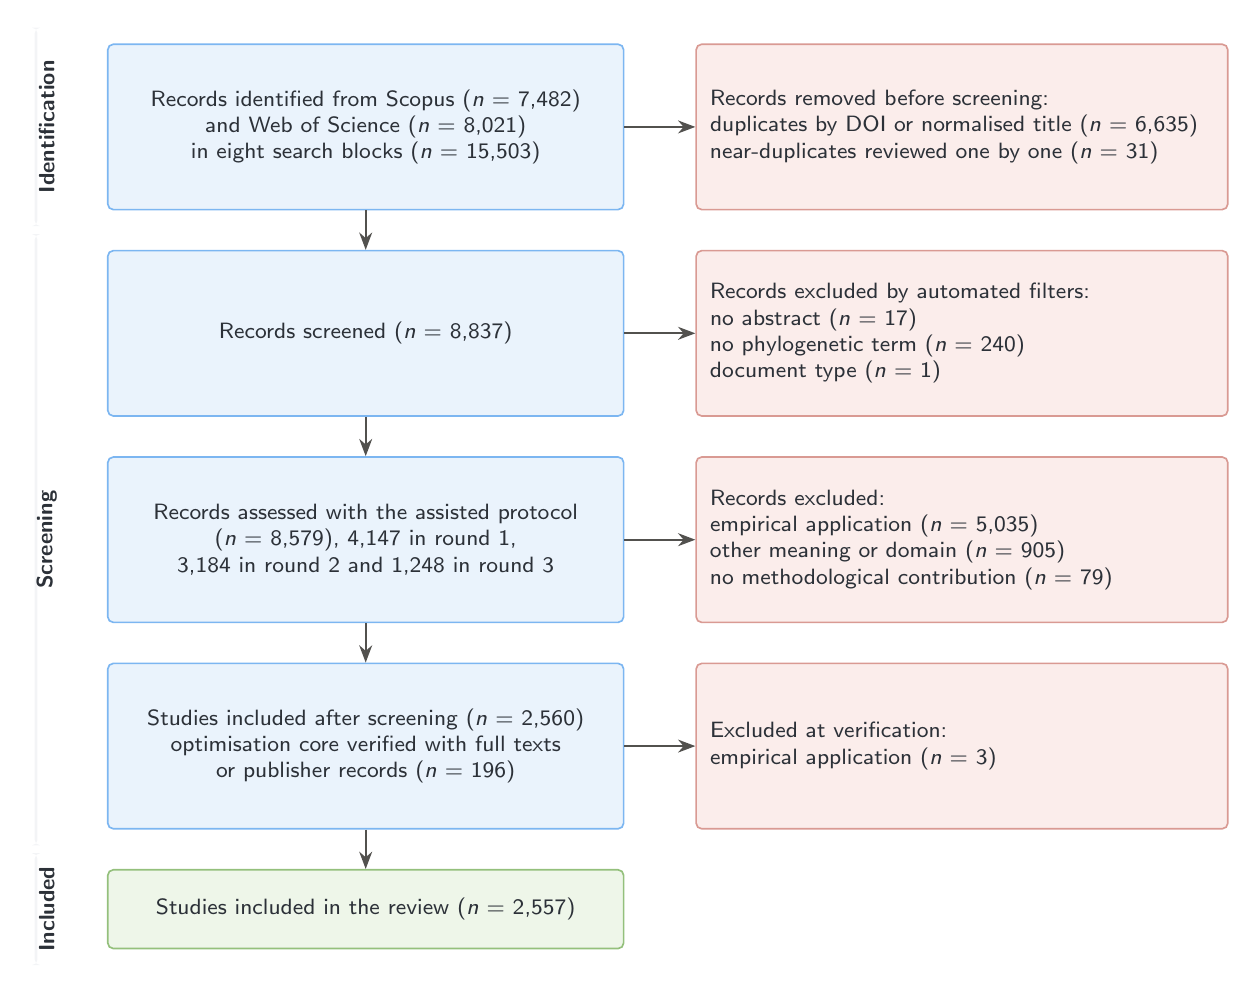
\begin{tikzpicture}[font=\footnotesize, text=ink, node distance=5mm and 9mm,
  main/.style={draw=pblueline, fill=pblue, rounded corners=2pt, align=center, text width=62mm, inner sep=5pt, line width=0.6pt, minimum height=21mm},
  excl/.style={draw=proseline, fill=prose, rounded corners=2pt, align=left, text width=64mm, inner sep=5pt, line width=0.6pt, minimum height=21mm},
  inc/.style={draw=pgreenline, fill=pgreen, rounded corners=2pt, align=center, text width=62mm, inner sep=5pt, line width=0.6pt, minimum height=10mm},
  arr/.style={-{Stealth[length=2.2mm]}, draw=ink2, line width=0.6pt}]
\node[main] (id) {Records identified from Scopus (\textit{n} = 7,482)\\ and Web of Science (\textit{n} = 8,021)\\ in eight search blocks (\textit{n} = 15,503)};
\node[excl, right=of id] (dup) {Records removed before screening:\\ duplicates by DOI or normalised title (\textit{n} = 6,635)\\ near-duplicates reviewed one by one (\textit{n} = 31)};
\node[main, below=of id] (scr) {Records screened (\textit{n} = 8,837)};
\node[excl, right=of scr] (aut) {Records excluded by automated filters:\\ no abstract (\textit{n} = 17)\\ no phylogenetic term (\textit{n} = 240)\\ document type (\textit{n} = 1)};
\node[main, below=of scr] (ass) {Records assessed with the assisted protocol\\ (\textit{n} = 8,579), 4,147 in round 1,\\ 3,184 in round 2 and 1,248 in round 3};
\node[excl, right=of ass] (exc) {Records excluded:\\ empirical application (\textit{n} = 5,035)\\ other meaning or domain (\textit{n} = 905)\\ no methodological contribution (\textit{n} = 79)};
\node[main, below=of ass] (ver) {Studies included after screening (\textit{n} = 2,560)\\ optimisation core verified with full texts\\ or publisher records (\textit{n} = 196)};
\node[excl, right=of ver] (exv) {Excluded at verification:\\ empirical application (\textit{n} = 3)};
\node[inc, below=of ver] (inc) {Studies included in the review (\textit{n} = 2,557)};
\draw[arr] (id) -- (scr); \draw[arr] (scr) -- (ass); \draw[arr] (ass) -- (ver); \draw[arr] (ver) -- (inc);
\draw[arr] (id) -- (dup); \draw[arr] (scr) -- (aut); \draw[arr] (ass) -- (exc); \draw[arr] (ver) -- (exv);
\begin{scope}[on background layer]
\node[fill=pband, rounded corners=2pt, fit={($(id.north west)+(-9mm,2mm)$) ($(id.south west)+(-9mm,-2mm)$)}, inner sep=0pt] (b1) {};
\node[fill=pband, rounded corners=2pt, fit={($(scr.north west)+(-9mm,2mm)$) ($(ver.south west)+(-9mm,-2mm)$)}, inner sep=0pt] (b2) {};
\node[fill=pband, rounded corners=2pt, fit={($(inc.north west)+(-9mm,2mm)$) ($(inc.south west)+(-9mm,-2mm)$)}, inner sep=0pt] (b3) {};
\end{scope}
\node[rotate=90, font=\footnotesize\bfseries] at ($(b1.west)+(1.6mm,0)$) {Identification};
\node[rotate=90, font=\footnotesize\bfseries] at ($(b2.west)+(1.6mm,0)$) {Screening};
\node[rotate=90, font=\footnotesize\bfseries] at ($(b3.west)+(1.6mm,0)$) {Included};
\end{tikzpicture}
\end{document}
